 %%%%%%%%%%%%%%%%%%%%%%%%%%%%%%%%%%%%%%%%%%%%%%%%%%%%%%%%%%%%%%%%%%%%%%%%
% Plantilla TFG/TFM
% Escuela Politécnica Superior de la Universidad de Alicante
% Realizado por: Jose Manuel Requena Plens
% Contacto: info@jmrplens.com / Telegram:@jmrplens
%%%%%%%%%%%%%%%%%%%%%%%%%%%%%%%%%%%%%%%%%%%%%%%%%%%%%%%%%%%%%%%%%%%%%%%%

\chapter{Metodología}
\label{metodologia}
\par El desarrollo de este \gls{tfg} va a consistir en la creación de un script de Python que tenga como entradas los datos \gls{sar} de Sentinel-1, y como salida la función de densidad de probabilidad para la \gls{bbch} y/o altura de la planta, utilizando \gls{rfr} para realizar esta estimación. 
\section{Datos para análisis y modelado}
\par Los datos con los que contamos para el estudio constan de 7 parcelas de cultivo de arroz llamadas: Calogne, Ermita, Puntal, Mínima, Puebla, Reboso y Vega, situadas en Sevilla, provincia del suroeste de España, que están representadas en un mapa en la figura \ref{fig:parcel}. De ellas se disponen de los datos tanto de satélite como de mediciones en campo para los años 2017 y 2018. 
\\
\par Los datos de entrada de satélite de los que disponemos para estas 7 parcelas son los coeficientes de backscattering para polarizaciones VV y VH en unidades de dB, obtenidos de las imágenes \gls{sar} post-procesadas de los satélites Sentinel-1. De ellos se emplean estos dos datos en dB, su diferencia en dB y la desviación estándar de todos los anteriores. Los datos tienen un periodo de revista de Sentinel-1 es de 6 días, lo que aporta una resolución temporal de cada ciclo de desarrollo aceptable. La cantidad de datos obtenidos por este método es limitada debido al reciente desarrollo del programa Copérnico. Aún así, parece válida para una aproximación suficientemente fiable, en comparación con los periodos de 12 días de los datos anteriores a 2016.
\\
\par Para realizar el modelo de observación necesitamos contrastar con datos reales tomados en tierra de los mismos cultivos, por lo que se recogen también de los siguientes datos de las 7 parcelas: su posición geográfica, área, fechas de siembra y de cosecha, producción, \gls{bbch} total, mínima y máxima, la altura media del cultivo y los días del año para los cuales se han tomado estos datos. De todos ellos, los más relevantes para este estudio son la \gls{bbch} por parcela, la altura del cultivo, por su relación con el desarrollo del cultivo para este caso, y las fechas de siembra, cosecha y de toma de datos, los cuáles no tienen porqué coincidir con el periodo de revista de los satélites de Sentinel-1.  Los periodos de cultivo del arroz son de aproximadamente 4 meses, disponemos de una cosecha por año y parcela, por lo que por cada época de cultivo se dispone de hasta 7 ciclos de desarrollo del cultivo, valor no muy amplio. En el caso de no disponer de suficiente información, esta se podría generar de manera estadística, partiendo de la original. 
\begin{figure}[H]
    \centering
    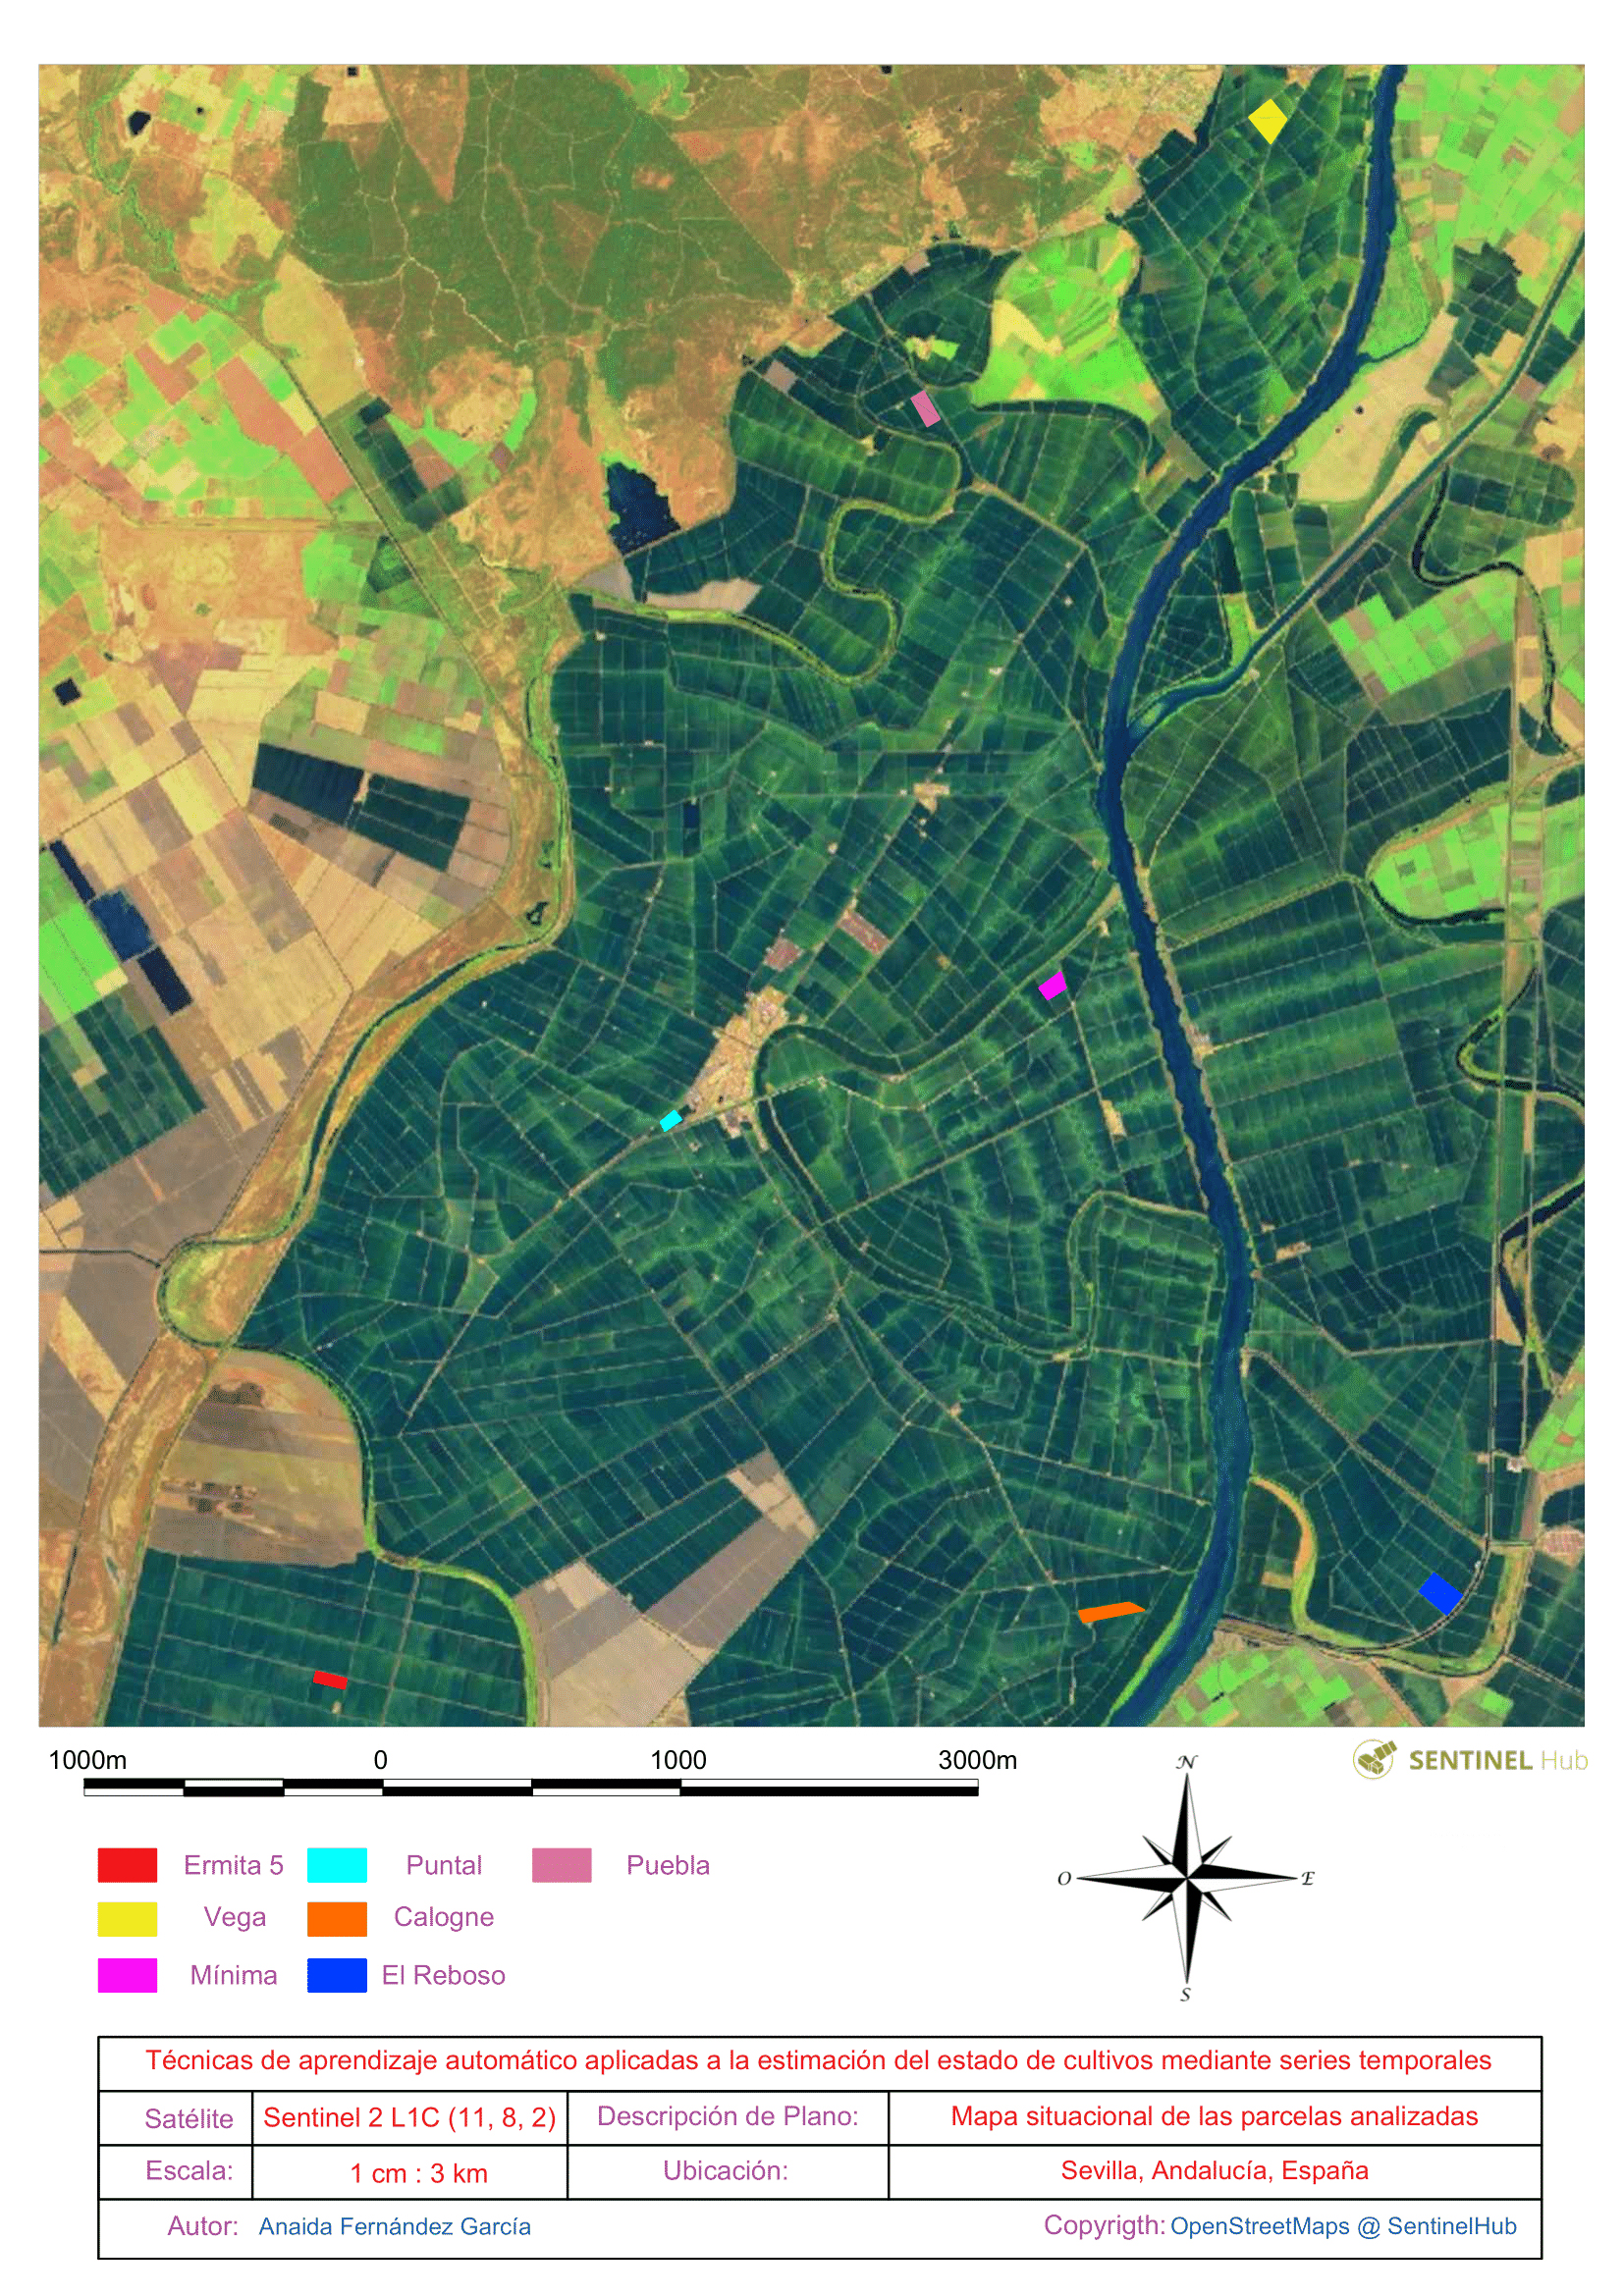
\includegraphics[height=20cm]{archivos/tfg/parcel_sat} % Tamaño de la imagen
    \caption{Mapa de la zona de estudio con las parcelas utilizadas destacadas. \cite{sentinelhub} }
    \label{fig:parcel}
\end{figure}
\section{Procesamiento y divisón de datos}
\par  El procesamiento que los datos de satélite necesitan para la elaboración del modelo es distinto dependiendo del método utilizado. En este proyecto se realizan pruebas para la estimación de 3 casos de salidas distintas: \gls{bbch}, altura (cm) y \gls{bbch} junto a altura (cm). Además, cada uno de estos casos se evalúa utilizando los datos de entrada a nivel de parcela (mediante la media) y a nivel de pixel, desconociendo a priori qué método obtiene mejores resultados. Para ambos métodos, el procesamiento de los datos comienza restringiendo la información al periodo que nos interesa: desde el día de siembra hasta el de cosecha. A continuación, se ajustan los días de los que se tiene información realizando una interpolación para los datos de \gls{bbch} y/o altura, haciéndolos coincidir con las fechas de toma de datos del satélite, cuyos datos no deben interpolarse ya que su evolución no es tan suave como la altura o la fenología. El siguiente procesamiento se da únicamente para el método a nivel de parcela: se calcula la media y la desviación estándar de los datos que vamos a utilizar como entradas del sistema (VV en dB, VH en dB, y el ratio entre ambos, VH-VV, también en dB). Si se está trabajando con el dato de altura, además, se realiza una limpieza de datos no válidos, ya que para algunas fechas concretas faltan datos de tierra con los que contrastar. 
\\
\par Para finalizar la preparación de los datos, se dividen estos en sets de entrenamiento y de test. La división se realiza por parcelas completas, para que sea más sencillo y completo su entrenamiento y posterior visualización. Para todos los casos se reservan 6 parcelas de entrenamiento y 1 de test de resultados, seleccionando este número y las parcelas concretas que mejor entrenan el sistema y optimizan los resultados. Los datos reales con los que se va a entrenar y examinar el modelo se preparan con la interpolación mencionada anteriormente y la división de parcelas que sigue los mismos requisitos que los datos de satélite. La única adaptación extra que tienen estos datos se da en el caso de nivel de pixel: como no contamos con la información medida en tierra a ese nivel de \gls{bbch} ni de altura, los valores generales para cada parcela interpolados deben ser asignados a cada uno de los píxeles correspondientes de esa parcela, es decir, todos los píxeles tendrán el mismo valor de salida para una misma parcela y día. Una interpretación gráfica aproximada de este procesamiento se puede ver en la figura *INSERTAR CROQUIS*.
\\
\par Una vez procesados todos los datos y creados los sets de entrenamiento y test, estos datos pueden ser guardados y cargados para no repetir el procesamiento en futuras ocasiones.
\section{Modelo de regresión y optimización}
\par A continuación, la implementación del regresor, su entrenamiento y evaluación, completa la creación del modelo de observación, estando listo para realizar predicciones. La técnica de regresión que se va a emplear es \gls{rfr}, una técnica de aprendizaje automático supervisado basada en árboles de decisión como se ha visto anteriormente y que ha sido probada su eficacia en generaciones de modelos similares para imágenes \gls{sar} en 2019 \cite{artRF}. En este caso, las salidas son los posibles valores de \gls{bbch} y/o la altura del cultivo, a los que se llega mediante decisiones sobre los rangos de valores que presentan los parámetros de entrada. Como todas las técnicas de aprendizaje automático, cuenta con una etapa de aprendizaje para la creación del modelo, y una etapa de test para comprobar su correcto funcionamiento. Normalmente, para cada vector de entrada, este modelo devuelve una salida única que es el estado fenológico o la altura más probable, pero por motivos de integración con el modelo de evolución, va a presentar la probabilidad para cada estado posible. 
\\
\par En la creación del modelo existen distintos parámetros modificables según la técnica de \gls{rfr} para optimizarlo acorde con las características del problema que se intenta resolver. El número de estimadores o número de árboles es uno de los principales parámetros, por defecto 100, el cual va representar el número de árboles de decisión de los que se va a componer el regresor. Mayor número de árboles implica una mayor complejidad y la posibilidad de generar soluciones más profundas y precisas, con el riesgo de hacer un sistema excesivamente complejo que tenga sobreajuste u overfitting en su entrenamiento y que tenga un coste computacional muy elevado sin realmente aportar mejoras significativas. Otros parámetros variables en la creación del regresor, ya dentro de los árboles de decisión, son la profundidad máxima (número máximo de nodos y niveles de cada árbol, por defecto nulo), el mínimo número de muestras para dividir un nodo interno (por defecto 2), el número mínimo de muestras para un nodo final (por defecto 1) o estado aleatorio inicial en la creación de los árboles de decisión (por defecto nulo), entre otros. Debido a las características de nuestro sistema, se mantienen los valores por defecto de todos los parámetros excepto el número de estimadores y el estado de aleatoriedad, parámetros que se destinan a la optimización del regresor ya que son los más influyentes en los resultados finales. 
\\
\par La optimización del número de estimadores se realiza ejecutando una prueba para todas las posibilidades entre los valores 1 y 1000 y escogiendo el valor mínimo de estimadores que presente un máximo local no puntual del error cuadrático, es decir, al que tiende de manera progresiva, y con una mejora considerable. La optimización del estado de aleatoriedad se realiza de la misma manera. Este último parámetro también garantiza una generación aleatoria similar para los mismos parámetros independientemente de las veces que se realicen las pruebas, esto es, la ``semilla'' de la que parte esta generación es la misma, por lo que se puede realizar una evaluación fiable de los resultados, ya que no van a depender de cómo se hayan generado inicialmente los árboles de decisión. 
\section{Evaluación de resultados}
\par Los resultados generales obtenidos para cada uno de los casos mencionados anteriormente, una vez optimizados los datos utilizados y los parámetros del regresor, se deben contrastar y evaluar para determinar la fiabilidad del modelo. Las evaluaciones de estos resultados se realizan con indicadores de error como la media del error absoluto (\gls{mae}), correpondiente a la fórmula \ref{eq:MAE}, la raíz del error cuadrático medio (\gls{rmse}), fómula \ref{eq:RMSE} o el coeficiente de determinación ($R^2$), fórmula \ref{eq:R2} para las predicciones del set de test, siendo las salidas del modelo una predicción de valor único.

\begin{equation}\label{eq:MAE}
\gls{mae} = \frac{\sum_{i=1}^{n} \left | y_i -x_i \right |}{n}
\end{equation} 
\begin{equation}\label{eq:RMSE}
\gls{rmse} = \sqrt{\frac{\sum_{i=1}^{n}(y_i- x_i )^2}{n}}
\end{equation}
\begin{equation}\label{eq:R2}
R^2 = \frac{\sigma^2_{xy}}{\sigma^2_x\sigma^2_y}
\end{equation}

\par Siendo $y_i$ los valores de salida predichos por el sistema y $x_i$ la verdad de tierra medida correspondiente para las fórmulas de \gls{mae} y \gls{rmse}. El coeficiente de determinación se calcularía según la fórmula \ref{eq:R2} siendo $\sigma_{xy}$ la covarianza de $x$ e $y$, valores predichos y contrastados; respectivamente, $\sigma^2_x$ la varianza de x y $\sigma^2_y$ la varianza de y. 
\\
\par Además, se evalúa también la influencia que ha tenido cada parámetro de entrada en las salidas, esto es, saber cuáles son los que presentan una mayor correlación con la variable de salida del sistema y por tanto son más útiles para su predicción. También se realizan representaciones gráficas comparativas entre las predicciones y los datos de tierra, de donde se puede observar para qué intervalos de la variable de salida el modelo funciona mejor.
%\par EVALUACIÖn DE ¡¡RESULTADOS!! (pdf) --> comparación con valores test&pred. comparación estaods fenológicos o alturas entre sí, mejor funcionamiento, etapas planas etc. R^2, RMSE. 